\documentclass{article}
\usepackage{graphicx}
\usepackage[top=2.5cm, bottom=3cm, left=2.5cm, right=2.5cm, headheight=41pt]{geometry}
\usepackage{fancyhdr}
\usepackage{lastpage}
\usepackage{hyperref}
\usepackage{caption}
\usepackage{amsmath,amssymb}
\usepackage{mathtools}
\usepackage[dvipsnames,table]{xcolor}
\definecolor{stemcol}{RGB}{30,100,20}
\usepackage[english]{babel}
\usepackage{titlesec}
\usepackage{listings}
\usepackage{longtable}
\usepackage{tikz}
\usepackage{enumitem}
\usepackage{booktabs}
\usepackage{float}
\usepackage{etoolbox}
\usepackage{algorithm}
\usepackage{algpseudocode}
\usepackage{array}

\hypersetup{
    colorlinks=false,
    pdfborder={0 0 0}
}

\definecolor{codegray}{RGB}{245,245,245}
\definecolor{codegreen}{rgb}{0,0.5,0}
\definecolor{codepurple}{rgb}{0.4,0,0.6}


\titleformat{\section}
  {\bfseries\Large}
  {\thesection}{1em}{}
\titleformat{\subsection}
  {\bfseries\large}
  {\thesubsection}{1em}{}
\titleformat{\subsubsection}
  {\bfseries\normalsize}
  {\thesubsubsection}{1em}{}

\lstdefinestyle{cppstyle}{
    language=C++,
    basicstyle=\ttfamily\small,
    keywordstyle=\color{codepurple}\bfseries,
    commentstyle=\color{codegreen},
    stringstyle=\color{orange!80!black},
    numberstyle=\tiny\color{gray},
    numbers=left,
    numbersep=8pt,
    frame=single,
    breaklines=true,
    tabsize=4,
    showstringspaces=false,
    backgroundcolor=\color{codegray}
}

\lstdefinestyle{bashstyle}{
    language=bash,
    basicstyle=\ttfamily\small,
    keywordstyle=\color{codepurple},
    commentstyle=\color{codegreen},
    frame=single,
    breaklines=true,
    numbers=none,
    backgroundcolor=\color{codegray}
}

\fancypagestyle{myfancy}{
    \fancyhf{}
    \renewcommand{\headrulewidth}{0.1pt}
    \renewcommand{\footrulewidth}{0.1pt}
    \lhead{
\includegraphics[height=1.3cm]{headerlogo.png}}
    \fancyhead[R]{\textbf{IF2211 Strategi Algoritma}\\
    Laporan Tugas Kecil 2\\
    \textit{Semester II 2025/2026}}
    \fancyfoot[R]{Halaman \thepage\ dari \pageref{LastPage}}
}

\addto\captionsenglish{
  \renewcommand{\bibname}{}
  \renewcommand{\refname}{}
}
\patchcmd{\thebibliography}{\section*{\refname}}{}{}{}
\patchcmd{\thebibliography}{\vspace*{-.5em}}{}{}{}

\begin{document}

\begin{titlepage}
\thispagestyle{empty}
\centering

\vspace{2em}
{\Large\bfseries Laporan Tugas Kecil 2\par}
\vspace{0.5em}
{\large\textsc{IF2211 Strategi Algoritma}\par}
{\normalsize\scshape Semester II Tahun 2025/2026\par}

\vspace{2em}


\includegraphics[width=0.5\textwidth]{cover.png}\\

\vspace{1.5em}
{Voxelization Objek 3D menggunakan Octree dengan Algoritma Divide and Conquer}\par
\vspace{2em}

{\large
Disusun Oleh:\\[0.5em]
\begin{tabular}{ll}
13524090 & Nashiruddin Akram \\
13524093 & Reinsen Silitonga \\
\end{tabular}
\par}

\vspace{6em}
{\large
\textsc{Program Studi Teknik Informatika}\\
\textsc{Sekolah Teknik Elektro dan Informatika}\\
\textsc{Institut Teknologi Bandung}\\[0.3em]
\normalsize Maret 2026\par}
\end{titlepage}

\thispagestyle{empty}
\vfill

\clearpage
\setlength{\headheight}{41pt}
\setlength{\headsep}{20pt}
\pagestyle{myfancy}
\setcounter{page}{1}
\tableofcontents
\newpage

\section{Algoritma Divide and Conquer}

\subsection{Gambaran Umum}

Algoritma melakukan \textit{surface voxelization} dengan pendekatan \textit{divide and conquer}
berbasis Octree. Model masukan dibaca sebagai kumpulan segitiga yang tersusun dari titik-titik
OBJ. Ruang 3D yang memuat model kemudian dibungkus oleh sebuah kubus akar. Kubus ini menjadi
node awal pada struktur Octree.

Pada setiap langkah rekursi, satu node kubus dievaluasi apakah masih berhubungan dengan
permukaan model. Jika tidak berhubungan, node tersebut dipangkas. Jika masih berhubungan dan
kedalaman belum mencapai batas, node dibagi menjadi delapan subkubus berukuran sama.
Jika kedalaman sudah mencapai batas, node tersebut dicetak sebagai satu voxel kubus pada
berkas keluaran.

Dengan strategi ini, program tidak menelusuri seluruh ruang secara merata. Program hanya
melanjutkan rekursi pada area yang dekat dengan permukaan objek, sehingga waktu komputasi
lebih efisien dibanding pembagian seragam tanpa \textit{pruning}.

\subsection{Langkah-langkah Algoritma}

\subsubsection{Membangun Root Bounding Box}

Sebelum rekursi dimulai, parser membaca semua baris \texttt{v} sebagai titik dan semua baris
\texttt{f} sebagai bidang segitiga. Pada saat membaca titik, program sekaligus menghitung nilai
minimum dan maksimum untuk sumbu $x$, $y$, dan $z$. Hasilnya adalah \textit{bounding box}
terkecil yang memuat seluruh model.

Karena Octree bekerja paling konsisten pada node berbentuk kubus, \textit{bounding box} awal
ditransformasi menjadi kubus dengan panjang sisi sama pada semua sumbu. Ukuran setengah sisi
kubus akar dihitung dengan rumus berikut:

\[
\text{half} = \max(\Delta x,\ \Delta y,\ \Delta z) \times 0.5 \times (1 + 10^{-4})
\]

Faktor $10^{-4}$ memberi \textit{padding} kecil agar kasus titik yang tepat berada di batas
kubus tidak mudah terpengaruh galat numerik.

\subsubsection{Divide: Membagi Kubus Menjadi 8 Oktant}

Untuk setiap node yang relevan dan belum mencapai kedalaman maksimum, kubus dibagi di titik
tengah ketiga sumbu:

\[
m_x = \frac{\min_x + \max_x}{2}, \quad
m_y = \frac{\min_y + \max_y}{2}, \quad
m_z = \frac{\min_z + \max_z}{2}
\]

Delapan oktant dibentuk dari kombinasi posisi kiri atau kanan, bawah atau atas, serta depan
atau belakang. Setiap oktant memiliki panjang sisi setengah dari node induk. Mekanisme ini
menghasilkan partisi ruang hierarkis yang tetap seragam pada setiap level.

\subsubsection{Memeriksa Irisan Permukaan}

Fungsi \texttt{buildOctree} memanggil fungsi deteksi irisan pada modul Octree untuk menentukan
apakah sebuah node masih memiliki keterkaitan dengan permukaan model. Pada implementasi ini,
uji dilakukan dengan pendekatan titik representatif untuk setiap bidang segitiga, yaitu tiga
titik sudut, tiga titik tengah sisi, dan satu titik pusat segitiga.

Sebuah bidang dianggap relevan terhadap node jika minimal satu titik representatifnya berada
di dalam \textit{bounding box} node. Jika tidak ada bidang yang relevan, node dinyatakan kosong
dan dihentikan dari rekursi.

Langkah ini adalah inti efisiensi algoritma. Ruang kosong tidak diwariskan ke level berikutnya,
sehingga jumlah node yang benar-benar diproses dapat berkurang secara signifikan.

\subsubsection{Conquer: Rekursi ke Oktant yang Relevan}

Untuk setiap oktant yang lolos filter, \texttt{buildOctree} dipanggil kembali dengan
\textit{bounding box} oktant sebagai domain baru. Nilai kedalaman dinaikkan dari
$d$ menjadi $d + 1$. Proses ini berlanjut sampai salah satu dari dua kondisi terpenuhi,
yaitu node dipangkas karena kosong, atau node mencapai kedalaman maksimum.

\subsubsection{Pembentukan Voxel sebagai Base Case}

Algoritma tidak akan terus membelah ruang selamanya. Kami membuat algoritma ini dengan memiliki dua kondisi berhenti (base case) 
yang mengontrol agar pembagian ini efisien dan menghasilkan output:

\begin{enumerate}
    \item \textbf{Pemangkasan Ruang Kosong (Pruning):} Sebelum membelah sebuah kotak, algoritma akan 
    mengecek apakah kotak tersebut memuat atau bersinggungan dengan minimal satu bagian (face) dari 
    model 3D aslinya menggunakan fungsi \texttt{punyaFace}. Jika kotak tersebut terbukti kosong (\texttt{!ok}), 
    maka pencarian di dalam cabang atau kotak tersebut dihentikan sepenuhnya. Ini mencegah algoritma 
    membuang-buang waktu memproses ruang udara kosong.
    
    \item \textbf{Mencapai Target Kedalaman Maksimal:} Jika pemotongan sudah mencapai target jumlah 
    kedalaman yang diinputkan oleh pengguna (\(d = md\)), algoritma menganggap bahwa ruang kecil itu 
    mewakili satu blok voxel yang valid. Pada tahap ini, algoritma mencetak bangun kubus tersebut 
    langsung ke dalam file output \texttt{.obj} melalui fungsi \texttt{printObjFile}, lalu proses 
    membelah dihentikan.
\end{enumerate}

\subsection{Pseudocode}

\begin{algorithm}
\caption{buildOctree}
\begin{algorithmic}[1]
\Procedure{buildOctree}{box, bidang, depth, maxDepth}
    \State catat statistik node pada depth

    \If{tidak ada bidang yang menyentuh box}
        \State catat statistik prune
        \State \Return
    \EndIf

    \If{$depth = maxDepth$}
        \State tulis 1 voxel kubus ke file OBJ
        \State \Return
    \EndIf

    \State $mid \gets center(box)$

    \For{setiap oktant $o$}
        \State \Call{buildOctree}{$o$, bidang, $depth+1$, maxDepth}
    \EndFor
\EndProcedure
\end{algorithmic}
\end{algorithm}

\subsection{Kompleksitas Waktu}

Analisis berikut hanya membahas kompleksitas waktu dalam notasi $O$. Misalkan $d$ adalah kedalaman maksimum Octree dan $N$ adalah jumlah bidang segitiga pada model
masukan. Pada setiap node, proses filter dapat memeriksa hingga $N$ bidang. Pada level ke-$k$,
jumlah node maksimum adalah $8^k$. Oleh karena itu, batas atas waktu total dapat ditulis sebagai:

\[
T(d) = O\left(\sum_{k=0}^{d-1} 8^k \cdot N\right) = O(8^d \cdot N)
\]

\section{Implementasi}

\subsection{Struktur File}

\begin{itemize}
    \item \texttt{bin/voxelizer.exe}: berkas executable hasil kompilasi.
    \item \texttt{bin/viewer.exe}: berkas executable untuk visualisasi model OBJ.
    \item \texttt{doc/Laporan\_Tucil2.pdf}: keluaran dokumen laporan.
    \item \texttt{src/geometry.hpp} dan \texttt{src/geometry.cpp}: struktur geometri dasar serta perhitungan bounding box.
    \item \texttt{src/parser.hpp} dan \texttt{src/parser.cpp}: parser OBJ dan pembentukan path keluaran.
    \item \texttt{src/octree.hpp} dan \texttt{src/octree.cpp}: rekursi octree, deteksi irisan, dan emisi voxel.
    \item \texttt{src/main.cpp}: antarmuka CLI, timer, dan laporan statistik.
    \item \texttt{src/viewer.hpp} dan \texttt{src/viewer.cpp}: modul visualisasi untuk menampilkan model hasil voxelization.
    \item \texttt{test/}: kumpulan data uji.
    \item \texttt{makefile}: aturan kompilasi dan pembersihan build.
\end{itemize}

\subsection{Modul Program}

\begin{table}[H]
\centering
\caption{Modul-modul program}
\begin{tabular}{lp{9cm}}
\toprule
\textbf{Modul} & \textbf{Fungsi} \\
\midrule
\texttt{geometry} & Struktur \texttt{Vec3}, \texttt{Box}/\texttt{BoundingBox}, dan \texttt{Triangle}; serta fungsi geometri dan bounding box \\
\texttt{parser}   & Membaca file \texttt{.obj} dengan validasi lengkap, menghasilkan path output \\
\texttt{octree}   & Deteksi irisan, emisi voxel, serta \texttt{buildOctree} secara rekursif \\
\texttt{main}     & Parsing argumen CLI, orkestrasi alur, timer proses, laporan terminal \\
\texttt{viewer}   & Menampilkan model OBJ hasil voxelization secara interaktif  \\
\bottomrule
\end{tabular}
\end{table}

\subsection{Validasi Input}

Program melakukan validasi menyeluruh pada file \texttt{.obj}:
\begin{itemize}
    \item Menolak titik dengan format tidak valid (kurang dari 3 koordinat).
    \item Menolak bidang non segitiga (lebih dari 3 titik).
    \item Menolak indeks bidang yang melebihi jumlah titik yang tersedia.
    \item Menolak indeks negatif.
    \item Prefix selain \texttt{v} dan \texttt{f} diabaikan (\texttt{vn}, \texttt{vt}, \texttt{\#}, dll.).
\end{itemize}

\subsection{Format Output}

Setiap voxel diekspor sebagai kubus dengan:
\begin{itemize}
    \item \textbf{8 titik} di sudut-sudut kubus.
    \item \textbf{12 bidang segitiga} (2 segitiga per sisi $\times$ 6 sisi), semua indeks positif.
    \item Ukuran kubus \textbf{seragam} (semua sisi sama panjang).
\end{itemize}

\section{Eksperimen dan Hasil}

\subsection{Hasil 1: Kubus pada depth 4}

\begin{figure}[H]
    \centering
    \IfFileExists{cube.png}{
        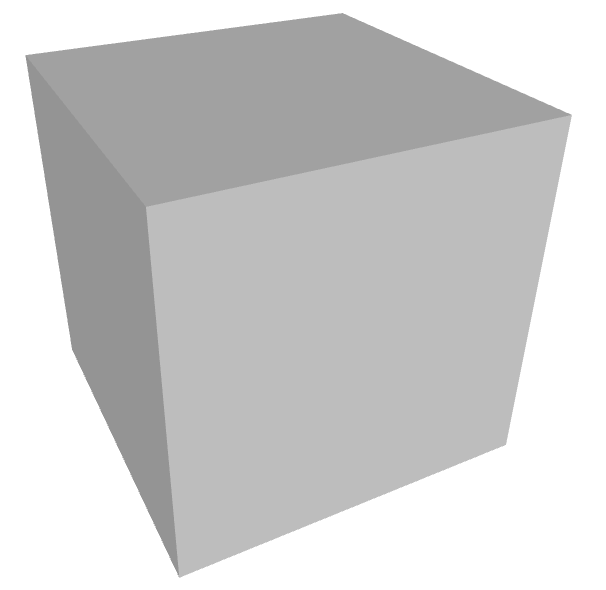
\includegraphics[width=0.9\textwidth]{cube.png}
    }{
        \fbox{\parbox[c][5cm][c]{0.85\textwidth}{\centering Gambar belum tersedia}}
    }
    \caption{Gambar input model kubus}
\end{figure}

\begin{figure}[H]
    \centering
    \IfFileExists{cube_depth4.png}{
        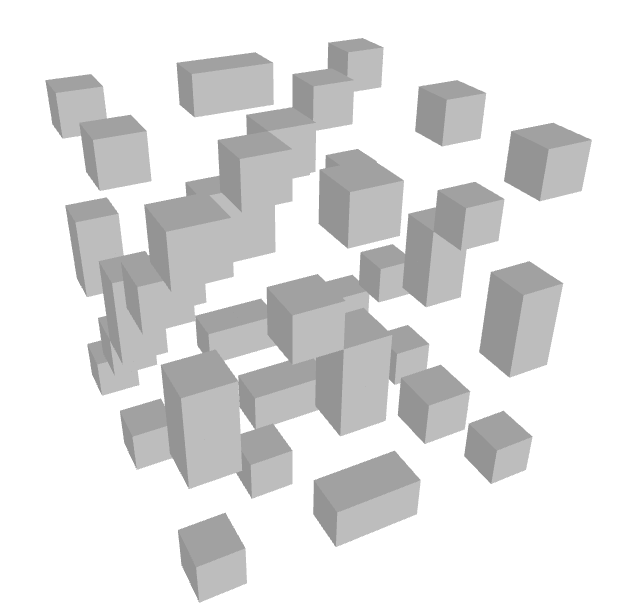
\includegraphics[width=0.9\textwidth]{cube_depth4.png}
    }{
        \fbox{\parbox[c][5cm][c]{0.85\textwidth}{\centering Gambar belum tersedia}}
    }
    \caption{Gambar output voxel kubus pada depth 4}
\end{figure}

\begin{lstlisting}[style=bashstyle, caption={Output terminal kubus pada depth 4}, captionpos=t]
$ ./bin/voxelizer.exe test/cube.obj 4
Berhasil membaca 8 vertex dan 12 face.
Membangun octree pada kedalaman 4...

Banyaknya voxel yang terbentuk   : 52
Banyaknya vertex yang terbentuk  : 416
Banyaknya faces yang terbentuk   : 624
Kedalaman octree                 : 4

Statistik node octree yang terbentuk:
1 : 1
2 : 8
3 : 64
4 : 360

Statistik node yang tidak perlu ditelusuri:
1 : 0
2 : 0
3 : 19
4 : 308

Lama waktu program berjalan      : 0.0018 s
Path file .obj disimpan          : test/cube-voxelized-4.obj

\end{lstlisting}

\subsection{Hasil 2: Line pada depth 3}

\begin{figure}[H]
    \centering
    \IfFileExists{line.png}{
        
\includegraphics[width=0.9\textwidth]{line.png}
    }{
        \fbox{\parbox[c][5cm][c]{0.85\textwidth}{\centering Gambar belum tersedia}}
    }
    \caption{Gambar input model line}
\end{figure}

\begin{figure}[H]
    \centering
    \IfFileExists{line_depth3.png}{
        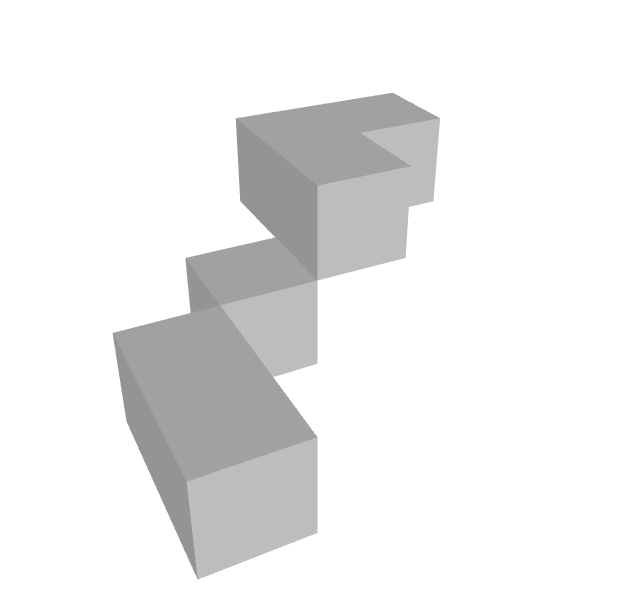
\includegraphics[width=0.9\textwidth]{line_depth3.png}
    }{
        \fbox{\parbox[c][5cm][c]{0.85\textwidth}{\centering Gambar belum tersedia}}
    }
    \caption{Gambar output voxel line pada depth 3}
\end{figure}

\begin{lstlisting}[style=bashstyle, caption={Output terminal line pada depth 3}, captionpos=t]
./bin/voxelizer.exe test/line.obj 3
Berhasil membaca 3 vertex dan 1 face.
Membangun octree pada kedalaman 3...

Banyaknya voxel yang terbentuk   : 6
Banyaknya vertex yang terbentuk  : 48
Banyaknya faces yang terbentuk   : 72
Kedalaman octree                 : 3

Statistik node octree yang terbentuk:
1 : 1
2 : 8
3 : 24

Statistik node yang tidak perlu ditelusuri:
1 : 0
2 : 5
3 : 18

Lama waktu program berjalan      : 0.0002 s
Path file .obj disimpan          : test/line-voxelized-3.obj

\end{lstlisting}

\subsection{Hasil 3: Pumpkin pada depth 5}

\begin{figure}[H]
    \centering
    \IfFileExists{pumpkin.png}{
        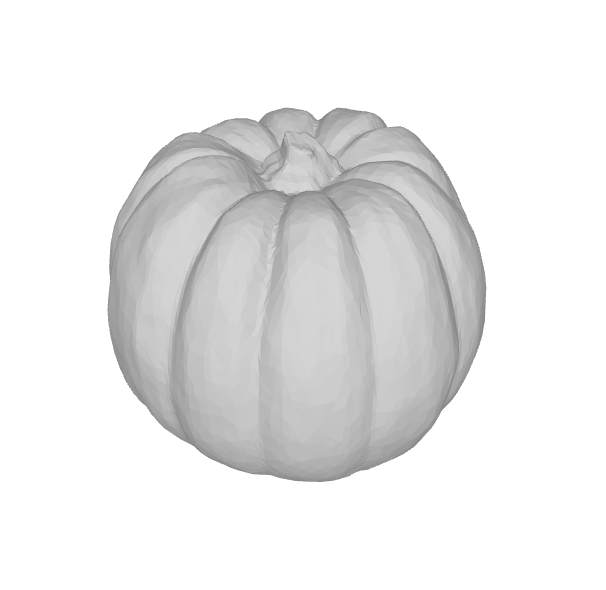
\includegraphics[width=0.9\textwidth]{pumpkin.png}
    }{
        \fbox{\parbox[c][5cm][c]{0.85\textwidth}{\centering Gambar belum tersedia}}
    }
    \caption{Gambar input model pumpkin}
\end{figure}

\begin{figure}[H]
    \centering
    \IfFileExists{pumpkin_depth5.png}{
        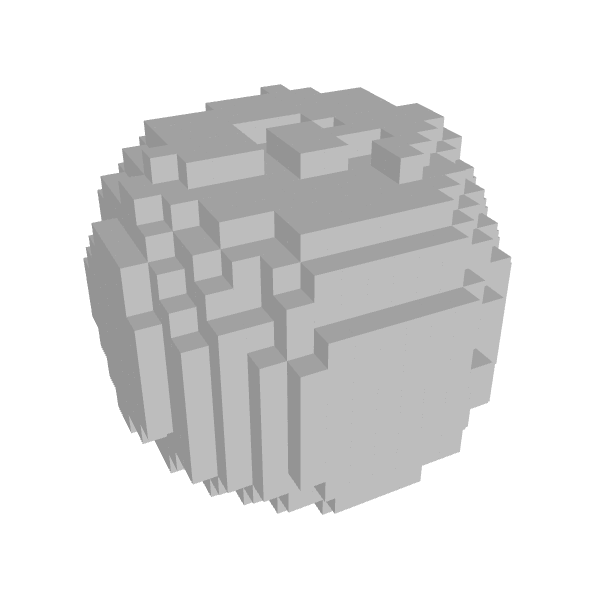
\includegraphics[width=0.9\textwidth]{pumpkin_depth5.png}
    }{
        \fbox{\parbox[c][5cm][c]{0.85\textwidth}{\centering Gambar belum tersedia}}
    }
    \caption{Gambar output voxel pumpkin pada depth 5}
\end{figure}

\begin{lstlisting}[style=bashstyle, caption={Output terminal pumpkin pada depth 5}, captionpos=t]
$ ./bin/voxelizer.exe test/pumpkin.obj 5
Berhasil membaca 5002 vertex dan 10000 face.
Membangun octree pada kedalaman 5...

Banyaknya voxel yang terbentuk   : 1049
Banyaknya vertex yang terbentuk  : 8392
Banyaknya faces yang terbentuk   : 12588
Kedalaman octree                 : 5

Statistik node octree yang terbentuk:
1 : 1
2 : 8
3 : 64
4 : 448
5 : 2144

Statistik node yang tidak perlu ditelusuri:
1 : 0
2 : 0
3 : 8
4 : 180
5 : 1095

Lama waktu program berjalan      : 0.3391 s
Path file .obj disimpan          : test/pumpkin-voxelized-5.obj

\end{lstlisting}

\subsection{Hasil 4: Pumpkin pada depth 7}

\begin{figure}[H]
    \centering
    \IfFileExists{pumpkin.png}{
        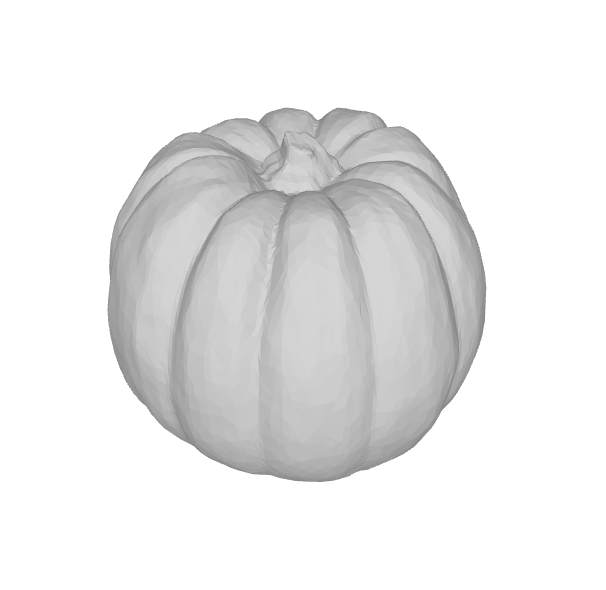
\includegraphics[width=0.9\textwidth]{pumpkin.png}
    }{
        \fbox{\parbox[c][5cm][c]{0.85\textwidth}{\centering Gambar belum tersedia}}
    }
    \caption{Gambar input model pumpkin}
\end{figure}

\begin{figure}[H]
    \centering
    \IfFileExists{pumpkin_depth7.png}{
        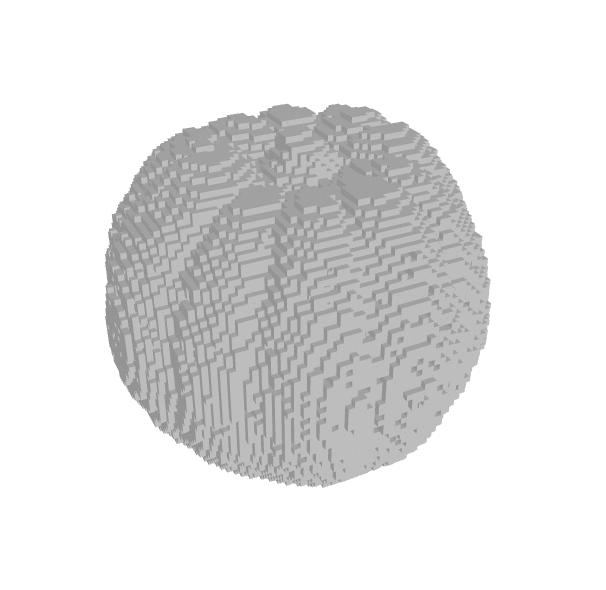
\includegraphics[width=0.9\textwidth]{pumpkin_depth7.png}
    }{
        \fbox{\parbox[c][5cm][c]{0.85\textwidth}{\centering Gambar belum tersedia}}
    }
    \caption{Gambar output voxel pumpkin pada depth 7}
\end{figure}

\begin{lstlisting}[style=bashstyle, caption={Output terminal pumpkin pada depth 7}, captionpos=t]
$ ./bin/voxelizer.exe test/pumpkin.obj 7
Berhasil membaca 5002 vertex dan 10000 face.
Membangun octree pada kedalaman 7...

Banyaknya voxel yang terbentuk   : 13270
Banyaknya vertex yang terbentuk  : 106160
Banyaknya faces yang terbentuk   : 159240
Kedalaman octree                 : 7

Statistik node octree yang terbentuk:
1 : 1
2 : 8
3 : 64
4 : 448
5 : 2144
6 : 8392
7 : 32368

Statistik node yang tidak perlu ditelusuri:
1 : 0
2 : 0
3 : 8
4 : 180
5 : 1095
6 : 4346
7 : 19098

Lama waktu program berjalan      : 5.3597 s
Path file .obj disimpan          : test/pumpkin-voxelized-7.obj

\end{lstlisting}

\subsection{Hasil 5: Cow pada depth 6}

\begin{figure}[H]
    \centering
    \IfFileExists{cow.png}{
        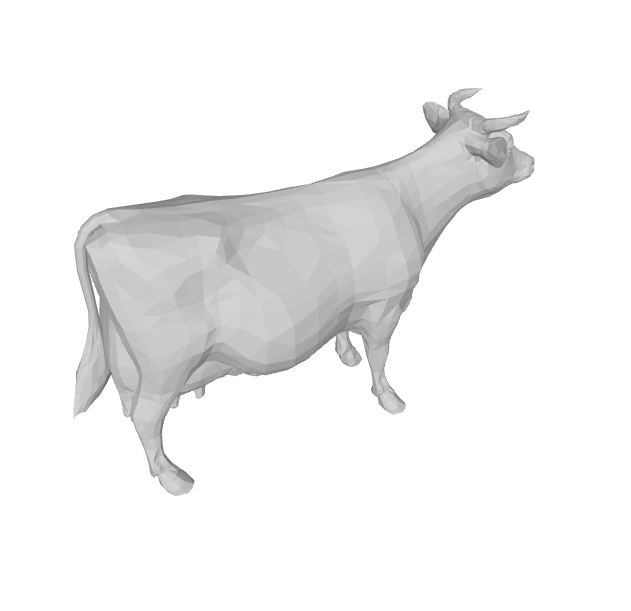
\includegraphics[width=0.9\textwidth]{cow.png}
    }{
        \fbox{\parbox[c][5cm][c]{0.85\textwidth}{\centering Gambar belum tersedia}}
    }
    \caption{Gambar input model cow}
\end{figure}

\begin{figure}[H]
    \centering
    \IfFileExists{cow_depth6.png}{
        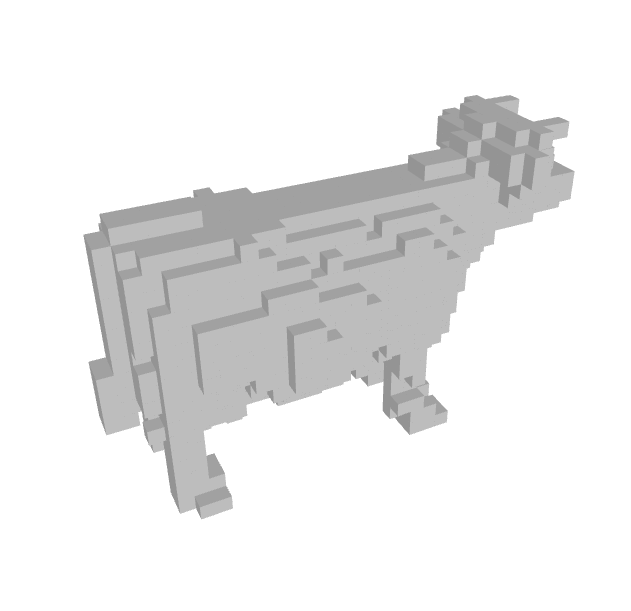
\includegraphics[width=0.9\textwidth]{cow_depth6.png}
    }{
        \fbox{\parbox[c][5cm][c]{0.85\textwidth}{\centering Gambar belum tersedia}}
    }
    \caption{Gambar output voxel cow pada depth 6}
\end{figure}

\begin{lstlisting}[style=bashstyle, caption={Output terminal cow pada depth 6}, captionpos=t]
$ ./bin/voxelizer.exe test/cow.obj 6
Berhasil membaca 4583 vertex dan 5804 face.
Membangun octree pada kedalaman 6...

Banyaknya voxel yang terbentuk   : 1248
Banyaknya vertex yang terbentuk  : 9984
Banyaknya faces yang terbentuk   : 14976
Kedalaman octree                 : 6

Statistik node octree yang terbentuk:
1 : 1
2 : 8
3 : 64
4 : 160
5 : 688
6 : 2608

Statistik node yang tidak perlu ditelusuri:
1 : 0
2 : 0
3 : 44
4 : 74
5 : 362
6 : 1360

Lama waktu program berjalan      : 0.1927 s
Path file .obj disimpan          : test/cow-voxelized-6.obj

\end{lstlisting}

\subsection{Hasil 6: Cow pada depth 8}

\begin{figure}[H]
    \centering
    \IfFileExists{cow.png}{
        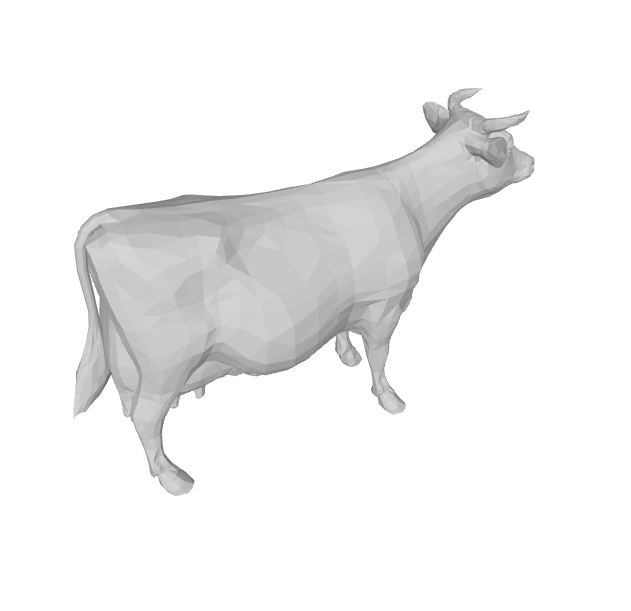
\includegraphics[width=0.9\textwidth]{cow.png}
    }{
        \fbox{\parbox[c][5cm][c]{0.85\textwidth}{\centering Gambar belum tersedia}}
    }
    \caption{Gambar input model cow}
\end{figure}

\begin{figure}[H]
    \centering
    \IfFileExists{cow_depth8.png}{
        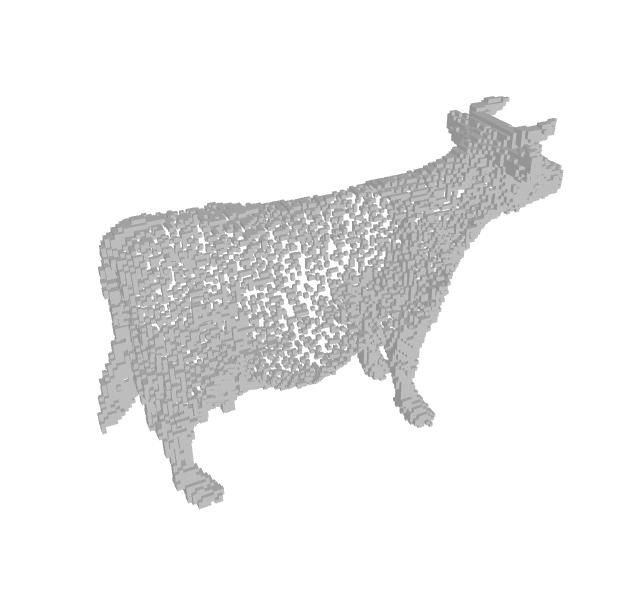
\includegraphics[width=0.9\textwidth]{cow_depth8.png}
    }{
        \fbox{\parbox[c][5cm][c]{0.85\textwidth}{\centering Gambar belum tersedia}}
    }
    \caption{Gambar output voxel cow pada depth 8}
\end{figure}

\begin{lstlisting}[style=bashstyle, caption={Output terminal cow pada depth 8}, captionpos=t]
$ ./bin/voxelizer.exe test/cow.obj 8
Berhasil membaca 4583 vertex dan 5804 face.
Membangun octree pada kedalaman 8...

Banyaknya voxel yang terbentuk   : 10205
Banyaknya vertex yang terbentuk  : 81640
Banyaknya faces yang terbentuk   : 122460
Kedalaman octree                 : 8

Statistik node octree yang terbentuk:
1 : 1
2 : 8
3 : 64
4 : 160
5 : 688
6 : 2608
7 : 9984
8 : 33896

Statistik node yang tidak perlu ditelusuri:
1 : 0
2 : 0
3 : 44
4 : 74
5 : 362
6 : 1360
7 : 5747
8 : 23691

Lama waktu program berjalan      : 2.5495 s
Path file .obj disimpan          : test/cow-voxelized-8.obj

\end{lstlisting}

\subsection{Hasil 7: Teapot pada depth 6}

\begin{figure}[H]
    \centering
    \IfFileExists{teapot.png}{
        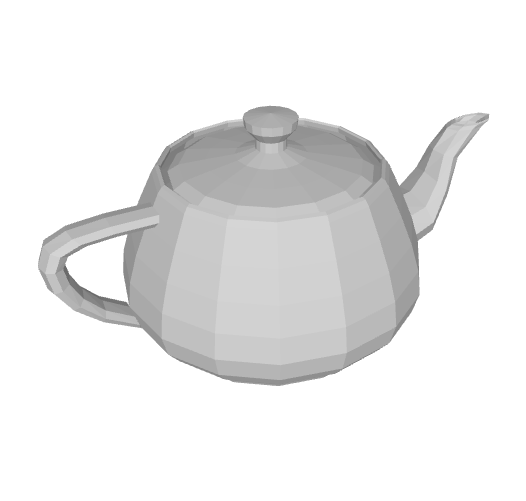
\includegraphics[width=0.9\textwidth]{teapot.png}
    }{
        \fbox{\parbox[c][5cm][c]{0.85\textwidth}{\centering Gambar belum tersedia}}
    }
    \caption{Gambar input model teapot}
\end{figure}

\begin{figure}[H]
    \centering
    \IfFileExists{teapot_depth6.png}{
        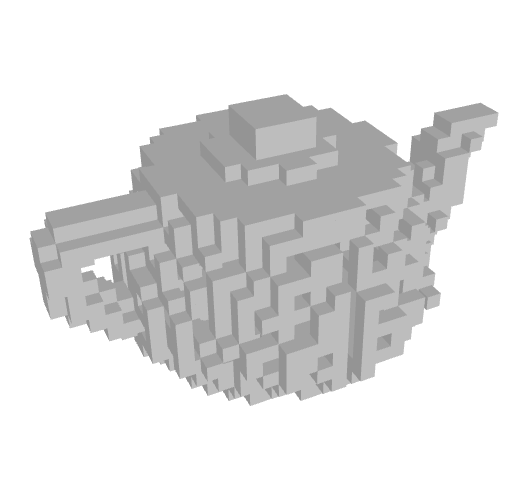
\includegraphics[width=0.9\textwidth]{teapot_depth6.png}
    }{
        \fbox{\parbox[c][5cm][c]{0.85\textwidth}{\centering Gambar belum tersedia}}
    }
    \caption{Gambar output voxel teapot pada depth 6}
\end{figure}

\begin{lstlisting}[style=bashstyle, caption={Output terminal teapot pada depth 6}, captionpos=t]
$ ./bin/voxelizer.exe test/teapot.obj 6
Berhasil membaca 530 vertex dan 1024 face.
Membangun octree pada kedalaman 6...

Banyaknya voxel yang terbentuk   : 1159
Banyaknya vertex yang terbentuk  : 9272
Banyaknya faces yang terbentuk   : 13908
Kedalaman octree                 : 6

Statistik node octree yang terbentuk:
1 : 1
2 : 8
3 : 64
4 : 192
5 : 800
6 : 2752

Statistik node yang tidak perlu ditelusuri:
1 : 0
2 : 0
3 : 40
4 : 92
5 : 456
6 : 1593

Lama waktu program berjalan      : 0.0774 s
Path file .obj disimpan          : test/teapot-voxelized-6.obj

\end{lstlisting}

\subsection{Hasil 8: Input Tidak Valid}

\begin{lstlisting}[style=bashstyle, caption={Output terminal input tidak valid}, captionpos=t]
\$ ./bin/voxelizer.exe test/teapot.obj abc
Error: kedalamanMaks harus berupa bilangan bulat positif
Penggunaan: ./bin/voxelizer.exe <input.obj> <kedalamanMaks>
  input.obj      : path ke file model 3D
  kedalamanMaks  : kedalaman octree (bilangan bulat >= 1, disarankan 4-8)

\end{lstlisting}

\clearpage
\section{Bonus Visualisasi}

Implementasi bonus ini berfokus pada pembuatan \textit{.obj viewer} interaktif
dalam bahasa C++. Viewer tersebut menampilkan model 3D hasil voxelization.
Implementasi viewer ini berada pada file \texttt{src/viewer.cpp} dan \texttt{src/viewer.hpp}.
Visualisasi digunakan sebagai validasi kualitatif agar bentuk objek,
kontur utama, dan distribusi voxel dapat ditinjau langsung dari berbagai
sudut pandang.

\subsection{Alur Rendering dan Interaksi}

\subsubsection{Membaca Model dan Menyiapkan Data Geometri}

Viewer membaca berkas OBJ hasil voxelization, kemudian memisahkan data menjadi daftar titik
(\textit{vertex}) dan daftar segitiga (\textit{face}). Pada tahap ini, struktur geometri disiapkan
sebagai data mentah yang akan diproses pada pipeline visualisasi.

\subsubsection{Normalisasi Model terhadap \textit{Bounding Box}}

Setelah data model terbaca, program menghitung \textit{bounding box} objek untuk mendapatkan
pusat model dan ukuran maksimum pada ketiga sumbu. Seluruh titik kemudian ditranslasi ke pusat
koordinat dan diskalakan agar dimensi model terjaga dalam rentang tampilan yang stabil.
Langkah ini membuat objek dengan ukuran berbeda tetap mudah ditampilkan dan diinteraksikan.

\subsubsection{Transformasi Ruang 3D ke Layar 2D}

Setiap titik model diputar pada sumbu $x$ dan $y$ sesuai sudut pandang pengguna.
Koordinat hasil rotasi lalu diproyeksikan ke koordinat layar 2D melalui fungsi proyeksi,
dengan faktor skala yang dipengaruhi oleh nilai \textit{zoom}. Dengan mekanisme ini,
perubahan sudut pandang dan pembesaran objek dapat terlihat secara langsung.

\subsubsection{Penyaringan, Pengurutan, dan Pewarnaan Segitiga}

Untuk setiap segitiga, program menghitung vektor normal permukaan sebagai dasar
penentuan visibilitas dan pencahayaan. Segitiga yang membelakangi kamera dipangkas
melalui \textit{back-face culling}. Segitiga yang tersisa kemudian diurutkan berdasarkan
kedalaman rata-rata (\textit{Painter's Algorithm}) agar tumpang tindih permukaan
ditampilkan lebih konsisten. Warna abu-abu tiap segitiga ditentukan dari orientasi normal
terhadap arah pandang, sehingga bentuk objek tampak lebih jelas.

\subsubsection{Interaksi Pengguna}

Interaksi utama yang didukung viewer adalah:

\begin{itemize}
    \item Klik dan \textit{drag} mouse untuk rotasi objek pada sumbu $x$ dan $y$.
    \item \textit{Scroll wheel} untuk \textit{zoom in} dan \textit{zoom out}.
\end{itemize}

\subsection{Perbandingan Visualisasi Web dan Visualizer C++}

Subbagian ini menampilkan tiga contoh perbandingan visualisasi antara hasil visualizer C++
dan viewer berbasis web.

Sumber viewer web yang digunakan:\\
\url{https://3dviewer.net/}

\subsubsection{Contoh 1: Objek Cow (depth 6)}

\begin{figure}[H]
    \centering
    \begin{minipage}[t]{0.48\textwidth}
        \centering
        \IfFileExists{cow_depth6.png}{
            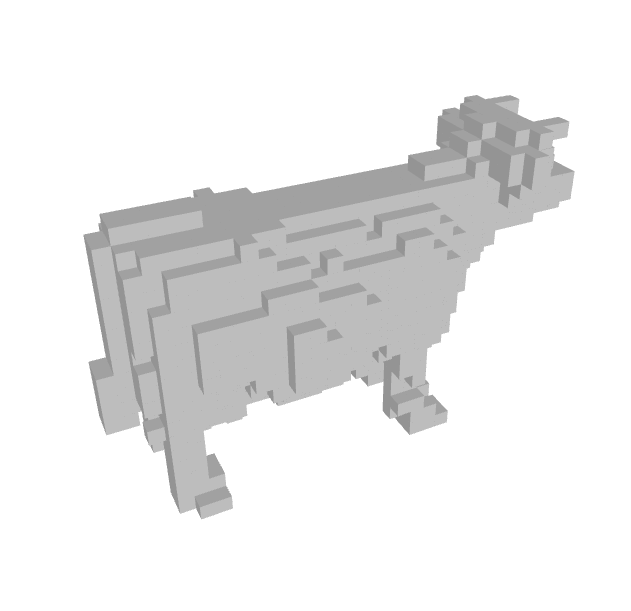
\includegraphics[width=\textwidth]{cow_depth6.png}
        }{
            \fbox{\parbox[c][4.3cm][c]{0.95\textwidth}{\centering Gambar web contoh 1 belum tersedia}}
        }
        \caption*{(a) Visualisasi web}
    \end{minipage}\hfill
    \begin{minipage}[t]{0.48\textwidth}
        \centering
        \IfFileExists{cow_depth6visualize.png}{
            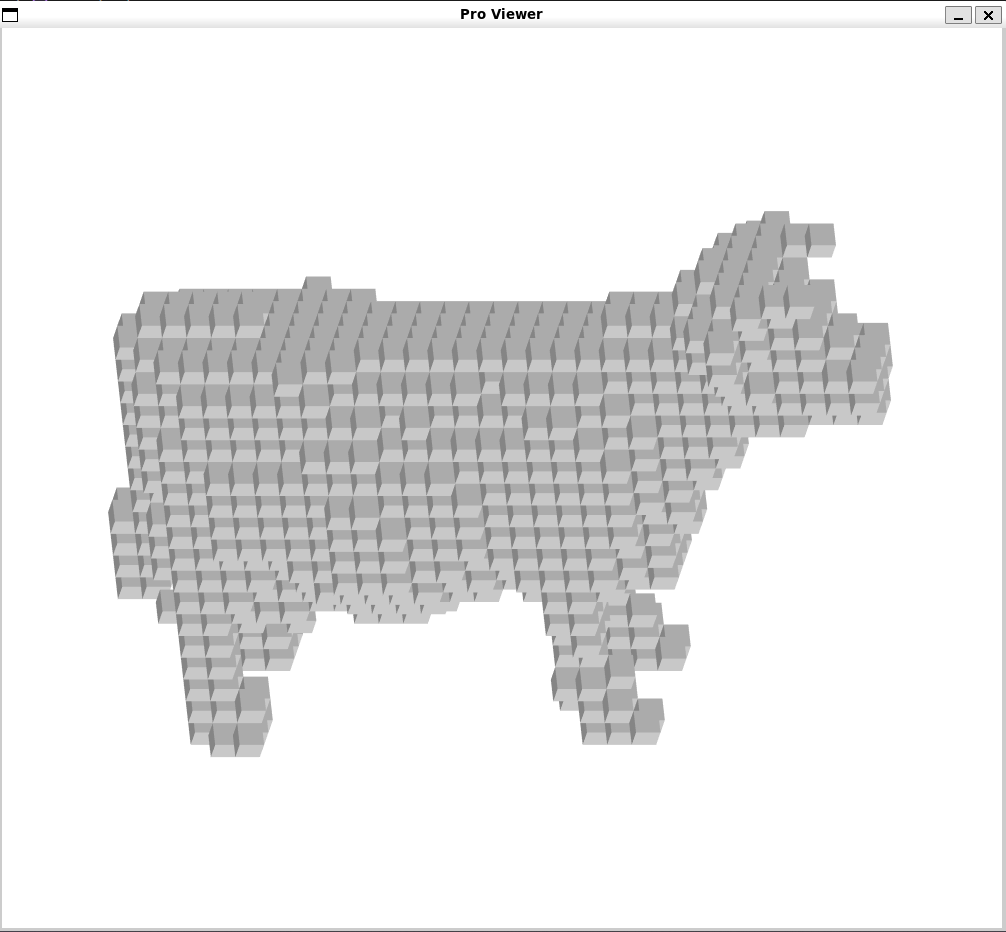
\includegraphics[width=\textwidth]{cow_depth6visualize.png}
        }{
            \fbox{\parbox[c][4.3cm][c]{0.95\textwidth}{\centering Gambar visualizer C++ contoh 1 belum tersedia}}
        }
        \caption*{(b) Visualizer C++}
    \end{minipage}
    \caption{Perbandingan contoh 1: visualisasi web dan visualizer C++ pada objek cow depth 6}
\end{figure}

\subsubsection{Contoh 2: Objek Pumpkin (depth 5)}

\begin{figure}[H]
    \centering
    \begin{minipage}[t]{0.48\textwidth}
        \centering
        \IfFileExists{pumpkin_depth5.png}{
            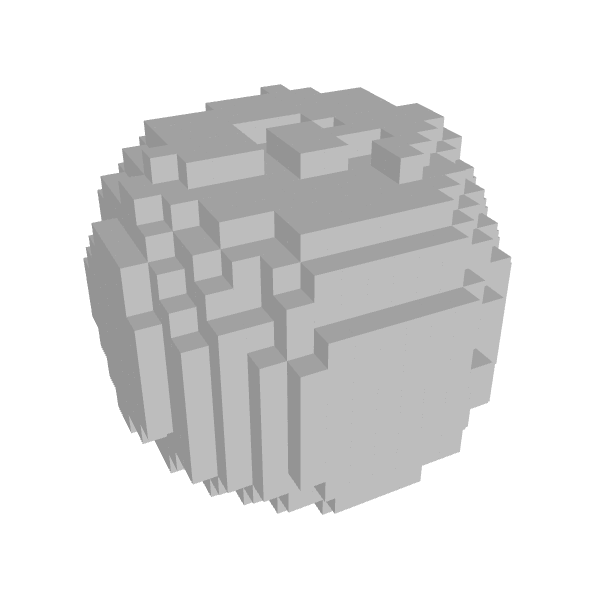
\includegraphics[width=\textwidth]{pumpkin_depth5.png}
        }{
            \fbox{\parbox[c][4.3cm][c]{0.95\textwidth}{\centering Gambar web contoh 2 belum tersedia}}
        }
        \caption*{(a) Visualisasi web}
    \end{minipage}\hfill
    \begin{minipage}[t]{0.48\textwidth}
        \centering
        \IfFileExists{pumpkin_depth5visualize.png}{
            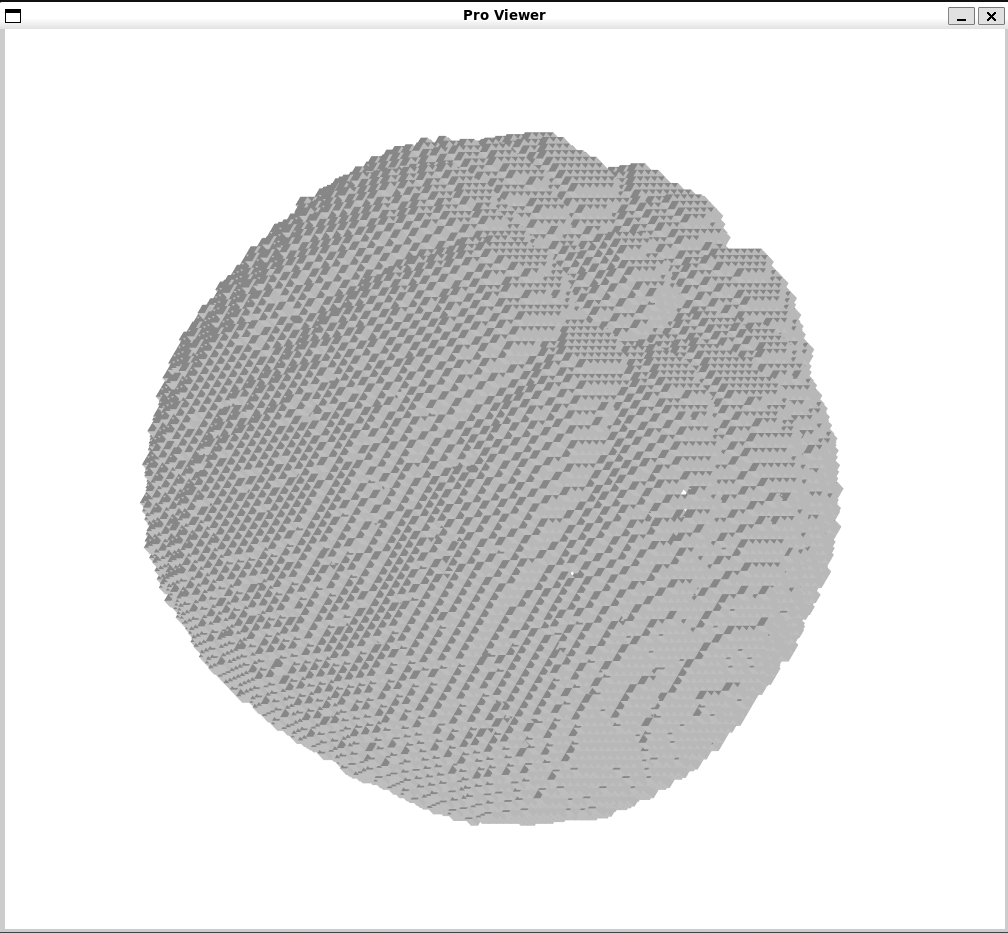
\includegraphics[width=\textwidth]{pumpkin_depth5visualize.png}
        }{
            \fbox{\parbox[c][4.3cm][c]{0.95\textwidth}{\centering Gambar visualizer C++ contoh 2 belum tersedia}}
        }
        \caption*{(b) Visualizer C++}
    \end{minipage}
    \caption{Perbandingan contoh 2: visualisasi web dan visualizer C++ pada objek pumpkin depth 5}
\end{figure}


\subsubsection{Contoh 3: Objek Teapot (depth 7)}

\begin{figure}[H]
    \centering
    \begin{minipage}[t]{0.48\textwidth}
        \centering
        \IfFileExists{teapot_depth7.png}{
            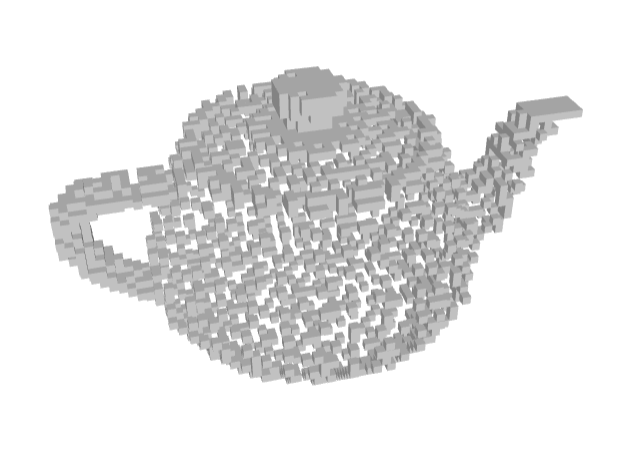
\includegraphics[width=\textwidth]{teapot_depth7.png}
        }{
            \fbox{\parbox[c][4.3cm][c]{0.95\textwidth}{\centering Gambar web contoh 3 belum tersedia}}
        }
        \caption*{(a) Visualisasi web}
    \end{minipage}\hfill
    \begin{minipage}[t]{0.48\textwidth}
        \centering
        \IfFileExists{teapot_depth7visualize.png}{
            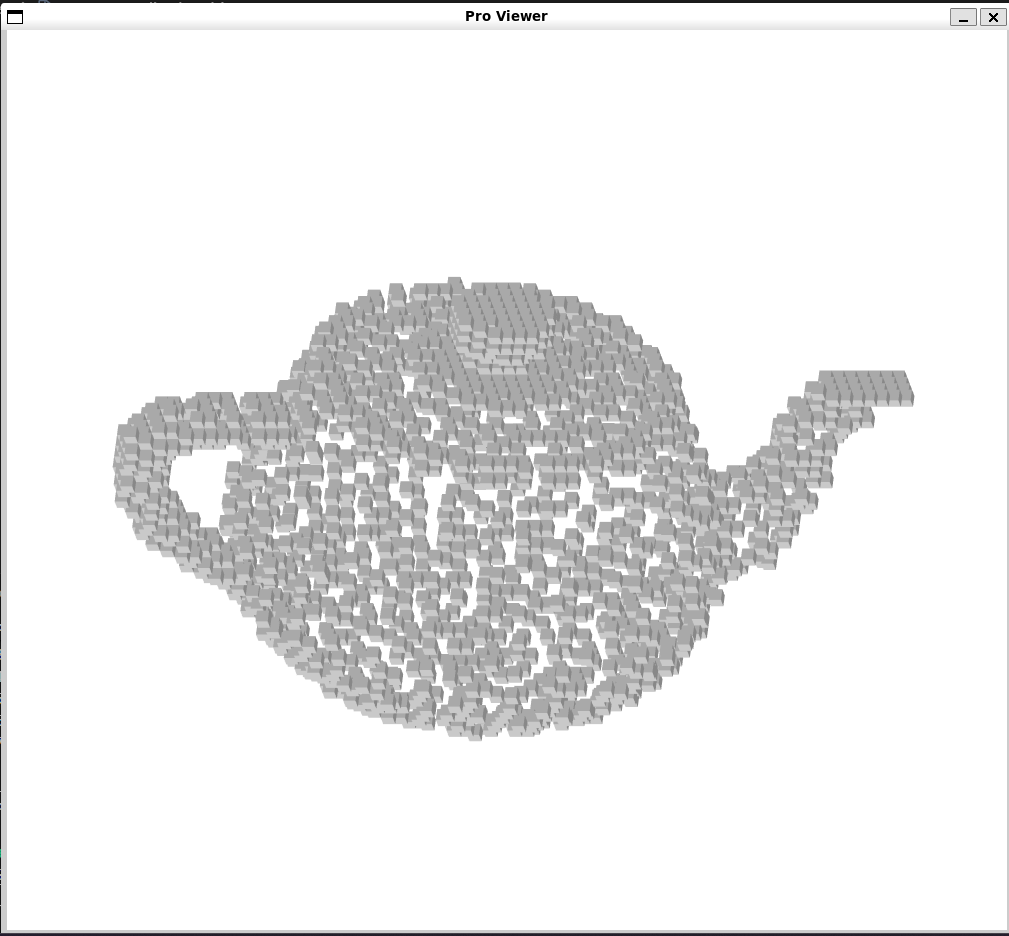
\includegraphics[width=\textwidth]{teapot_depth7visualize.png}
        }{
            \fbox{\parbox[c][4.3cm][c]{0.95\textwidth}{\centering Gambar visualizer C++ contoh 3 belum tersedia}}
        }
        \caption*{(b) Visualizer C++}
    \end{minipage}
    \caption{Perbandingan contoh 3: visualisasi web dan visualizer C++ pada objek teapot depth 7}
\end{figure}

\subsection{Perbandingan Umum}

Secara umum, kedua pendekatan menampilkan bentuk global objek voxel dengan konsisten.
Perbedaan utama terlihat pada batas antar-kubus yang saling bersisian. Pada visualisasi web,
garis di antara dua \textit{box} yang berdampingan cenderung hilang karena permukaan yang
berimpit dirender menyatu. Sebaliknya, pada visualizer C++ yang kami buat, garis pemisah
antar-kubus masih terlihat, sehingga struktur voxel diskret tampak lebih tegas.

\clearpage
\section{Lampiran}
\begin{itemize}
    \item Tautan Repository:\\
    \url{https://github.com/re1nsilitonga/Tucil2_13524090_13524093}
    \item Tabel Poin
    \begin{center}
    \renewcommand{\arraystretch}{1.5}
    \begin{tabular}{|c|p{9cm}|c|c|}
    \hline
    \textbf{No} & \textbf{Poin} & \textbf{Ya} & \textbf{Tidak} \\
    \hline

    1 & Program berhasil di kompilasi tanpa kesalahan & $\checkmark$ & $\square$ \\
    \hline

    2 & Program berhasil dijalankan & $\checkmark$ & $\square$ \\
    \hline

    3 & Hasil konversi .obj terdiri dari kubus-kubus kecil & $\checkmark$ & $\square$ \\
    \hline

    4 & Program informasi-informasi atau report & $\checkmark$ & $\square$ \\
    \hline

    5 & Program dapat menerima masukan .obj, dan mengembalikan output & $\checkmark$ & $\square$ \\
    \hline

    6 & [Bonus] Program menggunakan \textit{concurrency} & $\square$ & $\checkmark$ \\
    \hline

    7 & [Bonus] Program dapat menampilkan visualisasi .obj & $\checkmark$ & $\square$ \\
    \hline
    \end{tabular}
    \end{center}
    \item Pernyataan Tidak Melakukan Kecurangan
    \begin{center}
    \fbox{
    \begin{minipage}{0.9\textwidth}

    Tugas ini disusun sepenuhnya tanpa bantuan kecerdasan buatan (\textit{Generative AI}), 
    melainkan hasil pemikiran dan analisis mandiri.

    \vspace{1.5cm}

    \begin{flushright}

    
\includegraphics[width=3cm]{ttd1.jpeg}\\
    Nashiruddin Akram

    \vspace{1cm}

    
\includegraphics[width=3cm]{ttd2.png}\\
    Reinsen Silitonga

    \end{flushright}

    \end{minipage}
    }
    \end{center}
\end{itemize}
\clearpage

\end{document}